\section{Půllitr}

\begin{itemize}
    \item Obsah půllitru: \( V = \pi r^2 v = 0.5 \ \mathrm{l} = 0.5 \ \mathrm{dm}^3 \)
    \item Povrch půllitru: \( S = \pi r^2 + 2 \pi r v \)
\end{itemize}

Hledáme minimální povrch \( S \) půllitru při zadané podmínce.

\begin{enumerate}
    \item Vyjádříme z rovnice pro objem \( v \).
    \begin{align*}
        \pi r^2 v &= 0.5 \\
        v &= \frac{1}{2 \pi r^2}
    \end{align*}

    \item Dosadíme do rovnice pro povrch a upravíme.
    \begin{align*}
        S & = \pi r^2 + 2 \pi r v \\
        & = \pi r^2 + 2 \pi r \cdot \frac{1}{2 \pi r^2} \\
        & = \pi r^2 + \frac{1}{r}
    \end{align*}

    \item Hledáme minimum této funkce, využijeme tedy první derivace, kterou položíme rovnu nule a vyjádříme \( r \).
    \begin{align*}
        S' & = 0 \\
        2 \pi r - \frac{2}{r^2} & = 0 \quad (\text{hledáme } r > 0) \\
        2 \pi r^3 - 2 & = 0 \\
        \pi r^3 & = 1 \\
        r & = \sqrt[3]{\frac{1}{\pi}}
    \end{align*}

    \item Dosadíme vypočítané \( r \) do vyjádření \( v \) a dopočítáme hodnotu \( v \).
    \begin{align*}
        v & = \frac{1}{2 \pi r^2} \\
        v & = \frac{1}{2 \pi \sqrt[3]{\pi^{-1}}^2}
    \end{align*}
\end{enumerate}

Rozměry půllitru jsou poloměr \( r = \sqrt[3]{\frac{1}{\pi}} \) a výška \( v = \frac{1}{2 \pi \sqrt[3]{\pi^{-1}}^2} \).

\newpage

\section{Kelímek}

\begin{enumerate}
    \item V MATLABu napište funkci pro výpočet povrchu kelímku, jejímiž jedinými vstupními parametry budou \( r, R \) a \( V \).
    
    \lstinputlisting{matlab/povrch.m}
    
    \item Pro \( V = 0.6 \) vykreslete graf závislosti \( S \) na poloměru horní podstavy \( R \). Vykreslete závislost pro poloměry dolní podstavy \( r = \left\{ 0, 0.2, 0.4, 0.6, 0.8, 1 \right\} \). Výsledný graf vložte do zprávy. Odevzdejte i kód v MATLABu, který daný graf generuje.

    \begin{center}
    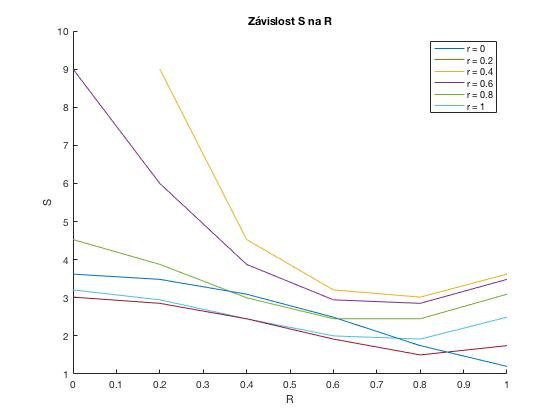
\includegraphics[width=0.73\textwidth]{matlab/plot1}
    \end{center}
    
    \begin{lstlisting}
r = 0:.2:1;
R = r;
v = 0.6;
        
hold on
for a = r
    y = povrch(a, R, v);
    plot(r, y);
end
hold off
    \end{lstlisting}
    
    \item Vykreslete 3D plochu závislosti \( S \) na \( r \) a \( R \) (\( r \) a \( R \) budou \( x \) a \( y \) osy grafu) pro hodnoty \( r \in \left[ 0.1, 1 \right] \) a \( R \in \left[ 0.1, 1 \right] \). Výsledný graf vložte do zprávy, kód odevzdejte.

    \begin{center}
        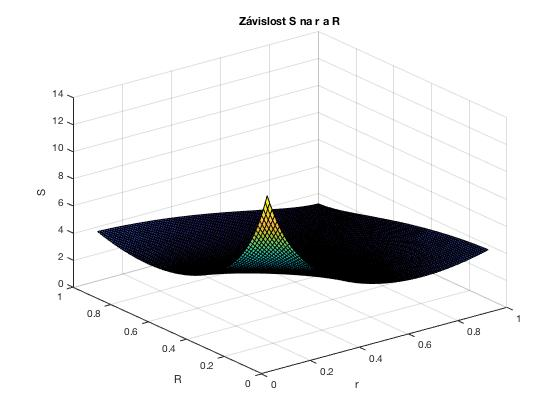
\includegraphics[width=0.73\textwidth]{matlab/plot2}
    \end{center}
    
    \begin{lstlisting}
r = .1:.01:1;
R = .1:.01:1;

[X, Y] = meshgrid(r, R);
Z = povrch(X, Y, 0.6);
surf(X, Y, Z);
    \end{lstlisting}
    
    \item Libovolnou metodou (s možností využití MATLABu) nalezněte řešení úlohy s přesností minimálně na 2 desetinná místa. Součástí odpovědi musí být i výsledná hodnota \( r, R, h \) a \( S \). MATLAB kód také odevzdejte.

    \begin{itemize}
        \item Poloměr spodní podstavy: 0.3860
        \item Poloměr horní podstavy: 0.7030
        \item Výška: 0.6265
        \item Povrch: 2.8702
    \end{itemize}
    
    \lstinputlisting{matlab/povrch_min.m}
    
    \item Krátce diskutujte, zda se kelímky takového tvaru skutečně používají a pokud ne, jaké mohou být případně jejich nevýhody.
    
    Kelímky tohoto rozměru se nevyrábějí, protože by připomínaly spíše talíře = byly by hodně široké a nízké, špatně by se z nich pilo.
\end{enumerate}

\newpage

\section{Maticová algebra}

\begin{enumerate}
    \item Dokažte, že pro každou čtvercovou matici \bf{A} platí:

    \begin{enumerate}
        \item \( \bf{A} + \bf{A}^T \) je symetrická.

        \bf{A} je symetrická, pokud \( a_{ij} = a_{ji} \).
        \begin{align*}
            \bf{B} &= \bf{A} + \bf{A}^T \\
            b_{ij} &= a_{ij} + a_{ji} \\
            b_{ji} &= a_{ji} + a_{ij} = a_{ij} + a_{ji} = b_{ij} \\
            & \Rightarrow \text{ matice \bf{B} je symetrická}
        \end{align*}

        \item \( \bf{A} - \bf{A}^T \) je antisymetrická.

        \bf{A} je symetrická, pokud \( a_{ij} = -a_{ji} \).
        \begin{align*}
            \bf{B} &= \bf{A} - \bf{A}^T \\
            b_{ij} &= a_{ij} - a_{ji} \\
            b_{ji} &= a_{ji} - a_{ij} = -a_{ij} + a_{ji} = -\left( a_{ij} - a_{ji} \right) = -b_{ij} \\
            & \Rightarrow \text{ matice \bf{B} je antisymetrická}
        \end{align*}

        \item existuje právě jedna symetrická matice \bf{B} a právě jedna antisymetrická matice \bf{C} tak, že  \( \bf{A} = \bf{B} + \bf{C} \).
        \item \( \bf{A}^T \cdot \bf{A} \) je symetrická.
    \end{enumerate}

    Označme \( \bf{B} = \frac{1}{2} \left( \bf{A} + \bf{A}^T \right) \) a \( \bf{C} = \frac{1}{2} \left( \bf{A} - \bf{A}^T \right) \). Potom
    \[
        \bf{B}^T = \left( \frac{1}{2} \left( \bf{A} + \bf{A}^T \right) \right)^T = \frac{1}{2} \left( \bf{A}^T + \bf{A} \right) = \frac{1}{2} \left( \bf{A} + \bf{A}^T \right) = \bf{B}
    \]
    matice \bf{B} je tedy symetrická. Podobně pro matici \bf{C} ukážeme
    \[
        \bf{C} = \left( \frac{1}{2} \left( \bf{A} - \bf{A}^T \right) \right)^T = \frac{1}{2} \left( \bf{A}^T - \bf{A} \right) = - \frac{1}{2} \left( \bf{A} - \bf{A}^T \right) = -\bf{C}
    \]
    že matice \bf{C} je antisymetrická. Zbývá dokázat jednoznačnost

    \begin{align*}
    \bf{A} + \bf{A}^T &= \bf{B} + \bf{B}^T + \bf{C} + \bf{C}^T \\
    &= \frac{1}{2} \left( \bf{A} + \bf{A}^T \right) + \frac{1}{2} \left( \bf{A} + \bf{A}^T \right) + \frac{1}{2} \lr{ \bf{A} - \bf{A}^T } - \frac{1}{2} \lr{ \bf{A} - \bf{A}^T } \\
    &= \frac{1}{2} \left( \bf{A} + \bf{A}^T \right) + \frac{1}{2} \left( \bf{A} + \bf{A}^T \right) \\
    &= 2 \cdot \bf{B} \\
    &= 2 \cdot \frac{1}{2} \cdot \lr{ \bf{A} + \bf{A}^T } \\
    &= \bf{A} + \bf{A}^T
    \end{align*}

    a

    \begin{align*}
    \bf{A} - \bf{A}^T &= \bf{B} - \bf{B}^T + \bf{C} - \bf{C}^T \\
    &= \frac{1}{2} \left( \bf{A} + \bf{A}^T \right) - \frac{1}{2} \left( \bf{A} + \bf{A}^T \right) + \frac{1}{2} \lr{ \bf{A} - \bf{A}^T } + \frac{1}{2} \lr{ \bf{A} - \bf{A}^T } \\
    &= \frac{1}{2} \left( \bf{A} - \bf{A}^T \right) + \frac{1}{2} \left( \bf{A} - \bf{A}^T \right) \\
    &= 2 \cdot \bf{C} \\
    &= 2 \cdot \frac{1}{2} \cdot \lr{ \bf{A} - \bf{A}^T } \\
    &= \bf{A} - \bf{A}^T
    \end{align*}

    \item Dokažte, že pokud je matice \( \bf{I} - \bf{A} \) regulární, pak \( \bf{A} \left( \bf{I} - \bf{A} \right)^{-1} = \left( \bf{I} - \bf{A} \right)^{-1} \bf{A} \).

    \begin{align*}
    \lr{ \bf{I} - \bf{A} }^{-1} \cdot \bf{A} &= \bf{A} \cdot \lr{ \bf{I} - \bf{A} }^{-1} \\
    \bf{A} &= \lr{\bf{I} - \bf{A}} \cdot \bf{A} \cdot \lr{ \bf{I} - \bf{A} }^{-1} \\
    \bf{A} &= \lr{\bf{A} - \bf{A}^2} \cdot \lr{\bf{I} - \bf{A}}^{-1} \\
    \bf{A} &= \bf{A} \cdot \lr{ \bf{I} - \bf{A} }^{-1} - \bf{A}^2 \cdot \lr{ \bf{I} - \bf{A} }^{-1} \\
    0 &= \bf{A} \cdot \lr{ \bf{I} - \bf{A} }^{-1} - \bf{A}^2 \cdot \lr{ \bf{I} - \bf{A} }^{-1} - \bf{A} \\
    0 &= \bf{A} \cdot \lr{ \lr{ \bf{I} - \bf{A} }^{-1} - \bf{A} \cdot \lr{ \bf{I} - \bf{A} }^{-1} - \bf{I} } \\
    0 &= \bf{A} \cdot \lr{ \lr{ \bf{I} - \bf{A} } \cdot \lr{ \bf{I} - \bf{A} }^{-1} -\bf{I} } \\
    0 &= \bf{A} \cdot  \lr{ \bf{I} - \bf{I} } \\
    0 &= \bf{A} \cdot 0 \\
    0 &= 0
    \end{align*}

    \item Dokažte, že pro každé \( \bf{A} \in \bbR^{m \times n} \) a \( \bf{B} \in \bbR^{n \times m} \) má matice 
    \[
        \bf{L} = 
        \begin{bmatrix}
            \bf{I} - \bf{B} \bf{A} & \bf{B} \\
            2 \bf{A} - \bf{A} \bf{B} \bf{A} & \bf{A} \bf{B} - \bf{I}
        \end{bmatrix}
    \]
    vlastnost \( \bf{L}^2 = \bf{I} \) (kde \( \bf{L}^2 \) je zkratka pro \( \bf{L} \bf{L} \)).

    Nejdříve je potřeba zkontrolovat, zda-li odpovídají vnitřní rozměry jednotlivých podmatic.
    \[
    \begin{bmatrix}
    n \cdot n & n \cdot m \\
    m \cdot n & m \cdot m
    \end{bmatrix}
    \cdot
    \begin{bmatrix}
    n \cdot n & n \cdot m \\
    m \cdot n & m \cdot m
    \end{bmatrix}
    \]
    z čehož je vidět, že vnitřní rozměry si odpovídají. Dále vypočteme jednotlivé prvky výsledné matice a porovnáme ji s maticí jednotkovou.
    
    \begin{align*}
    (\bf{I} - \bf{B}\bf{A}) \cdot (\bf{I} - \bf{B}\bf{A}) + \bf{B} \cdot (2\bf{A} - \bf{A}\bf{B}\bf{A}) &= \bf{I}^2 - 2\bf{B}\bf{A} + \bf{B}\bf{A}\bf{B}\bf{A} + 2\bf{B}\bf{A} - \bf{B}\bf{A}\bf{B}\bf{A} \\
    &= \bf{I}^2 \\
    &= \bf{I}
    \end{align*}
    
    \[
    (\bf{I} -\bf{B}\bf{A}) \cdot \bf{B} + \bf{B} \cdot (\bf{A}\bf{B} - \bf{I}) = \bf{B} \cdot \bf{B}\bf{A}\bf{B} + \bf{B}\bf{A}\bf{B} - \bf{B} = 0
    \]

    \begin{multline*}
    (2\bf{A} - \bf{A}\bf{B}\bf{A}) \cdot (\bf{I} - \bf{B}\bf{A}) + (\bf{A}\bf{B} - \bf{I}) \cdot (2\bf{A} - \bf{A}\bf{B}\bf{A}) = \\
    = 2\bf{A} - 2\bf{A}\bf{B}\bf{A} - \bf{A}\bf{B}\bf{A} + \bf{A}\bf{B}\bf{A}\bf{B}\bf{A} + 2\bf{A}\bf{B}\bf{A} - \bf{A}\bf{B}\bf{A}\bf{B}\bf{A} - 2\bf{A} + \bf{A}\bf{B}\bf{A} = 0
    \end{multline*}

    \begin{align*}
    (2\bf{A} - \bf{A}\bf{B}\bf{A}) \cdot \bf{B} + (\bf{A}\bf{B} - \bf{I}) \cdot (\bf{A}\bf{B} - \bf{I}) &= 2\bf{A}\bf{B} - \bf{A}\bf{B}\bf{A}\bf{B} + \bf{A}\bf{B}\bf{A}\bf{B} - \bf{A}\bf{B} - \bf{A}\bf{B} + \bf{I}^2  \\
    &= \bf{I}^2 \\
    &= \bf{I}
    \end{align*}

    %\[
     %   \begin{bmatrix}
      %      (\bf{I} - \bf{B}\bf{A}) \cdot (\bf{I} - \bf{B}\bf{A}) + \bf{B} \cdot (2\bf{A} - \bf{A}\bf{B}\bf{A}) & (\bf{I} -\bf{B}\bf{A}) \cdot \bf{B} + \bf{B} \cdot (\bf{A}\bf{B} - \bf{I}) \\
       %     (2\bf{A} - \bf{A}\bf{B}\bf{A}) \cdot (\bf{I} - \bf{B}\bf{A}) + (\bf{A}\bf{B} - \bf{I}) \cdot (2\bf{A} - \bf{A}\bf{B}\bf{A}) & (2\bf{A} - \bf{A}\bf{B}\bf{A}) \cdot \bf{B} + (\bf{A}\bf{B} - \bf{I}) \cdot (\bf{A}\bf{B} - \bf{I})
    %    \end{bmatrix}
     %   =
      %  \begin{bmatrix}
       % 1 & 0 \\
    %    0 & 1
     %   \end{bmatrix}
   % \]

    Vlastnost \( \bf{L}^2 = \bf{I} \) (kde \( \bf{L}^2 \) je zkratka pro \( \bf{L} \bf{L} \)) tedy platí.
\end{enumerate}